\documentclass{standalone}
\usepackage{flowchart}
\usepackage{tikz}
\usepackage{amssymb}

\begin{document}
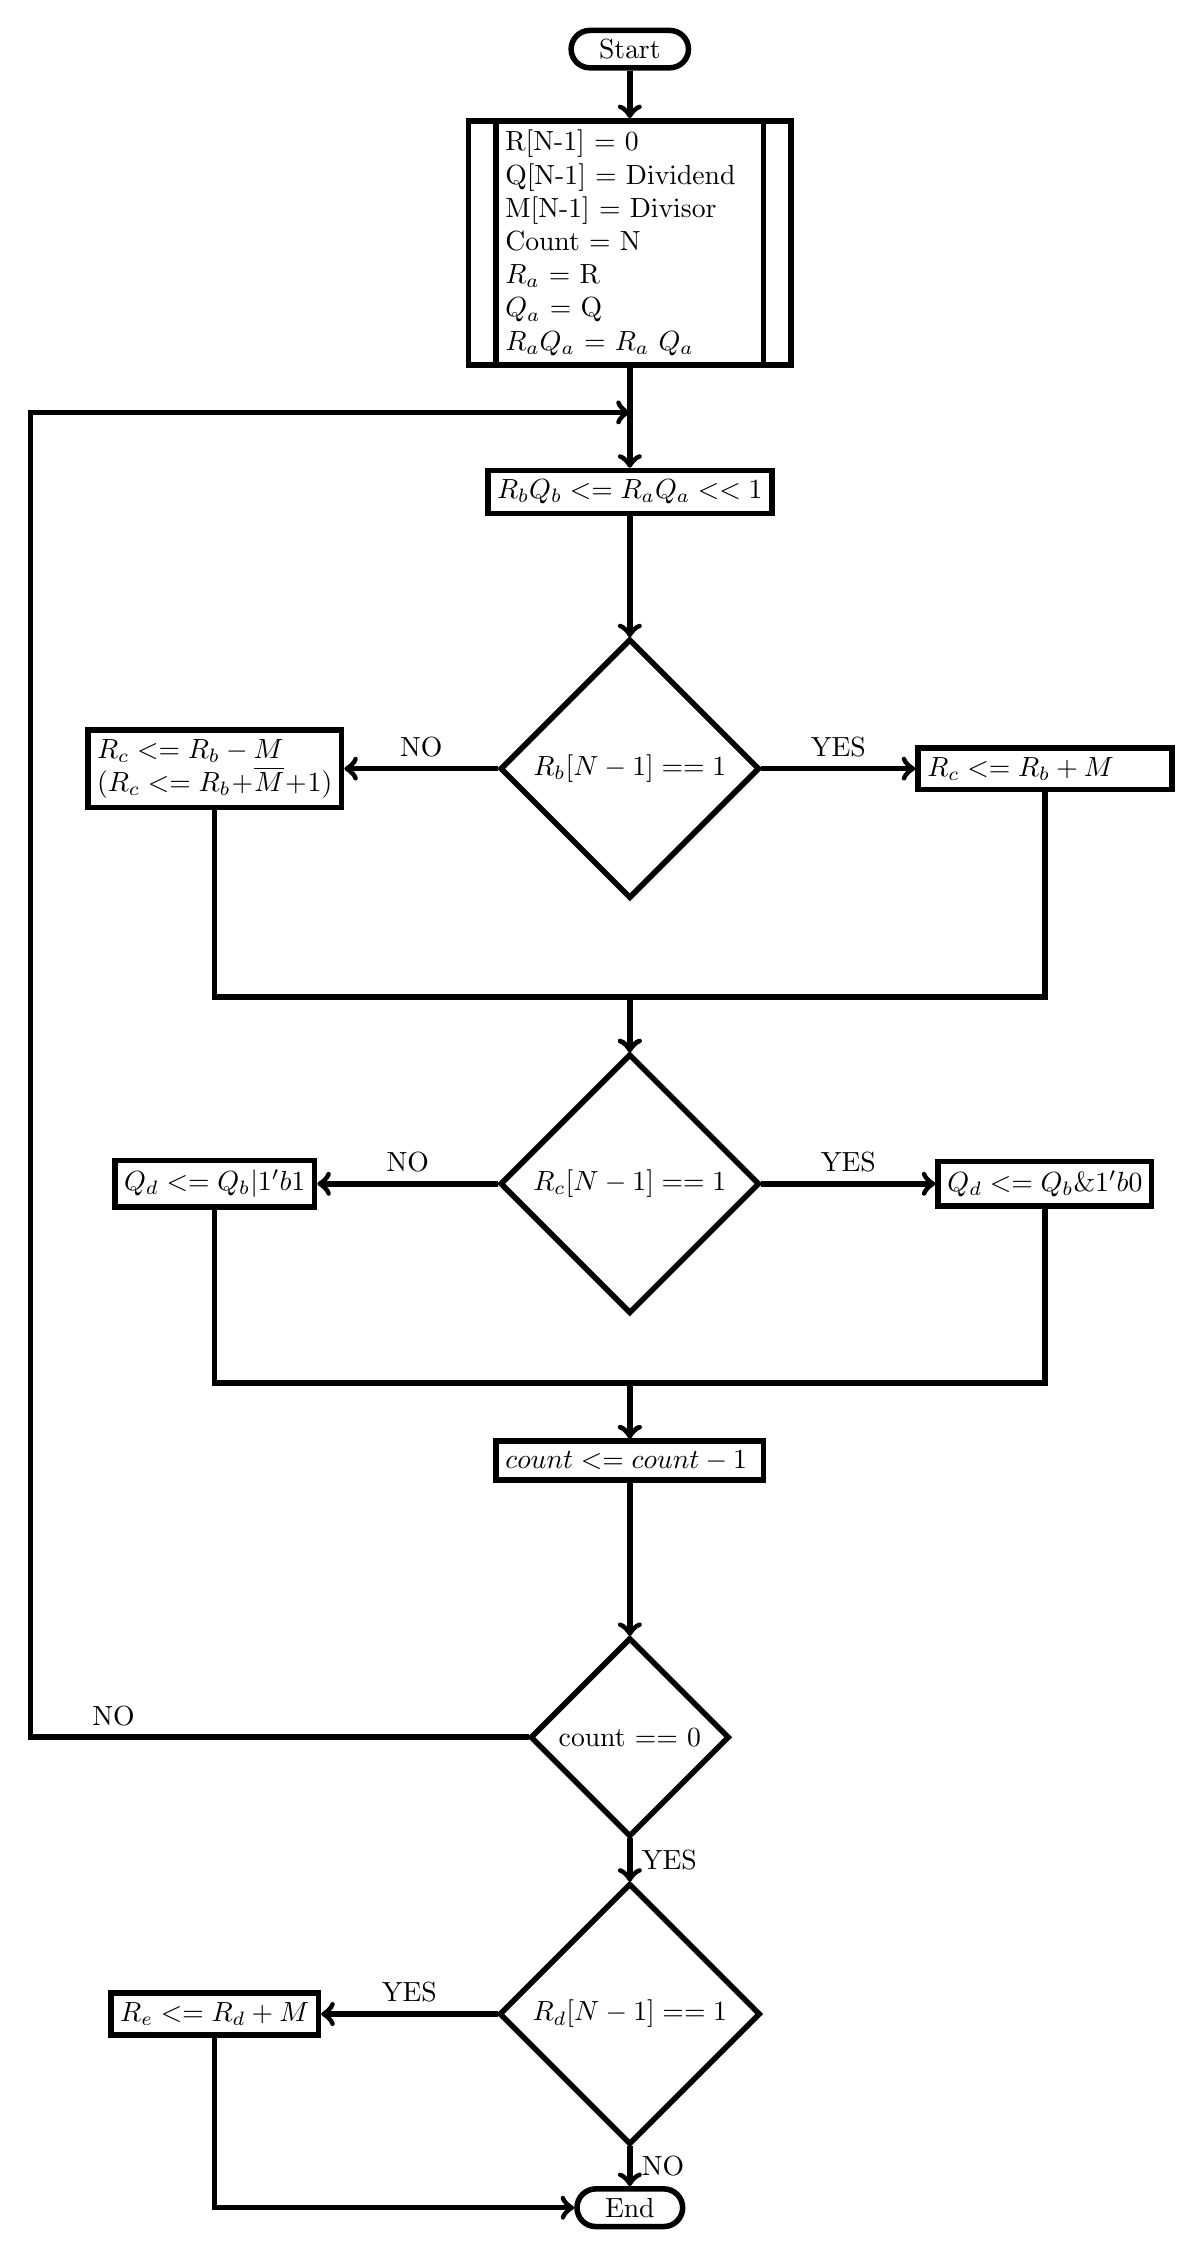
\begin{tikzpicture}[line width=0.2em]
    \node[draw, terminal] (st) at (0,0) {Start};

    \node[draw, predproc, text width=9em] (ini) at ([yshift=-7em]st) {R[N-1] = 0\\Q[N-1] = Dividend\\M[N-1] = Divisor\\Count = N\\ $R_a$ = R\\ $Q_a$ = Q\\ $R_aQ_a$ = {$R_a$ $Q_a$}};


    \node[draw, process] (comb) at ([yshift=-9em]ini) {$R_bQ_b <= R_aQ_a << 1$};

    \node[draw, decision] (dec3) at ([yshift=-10em]comb) {$R_b[N-1] == 1$};

    \node[draw, process, text width=8.5em] (sub1) at ([xshift=-15em,yshift=-0em]dec3) {$R_c <= R_b - M$\\ ($R_c <= R_b + \overline{M} + 1$)};
    \node[draw, process, text width=8.5em] (sub2) at ([xshift=15em,yshift=-0em]dec3) {$R_c <= R_b + M$};


    \node[draw, decision] (dec1) at ([yshift=-15em]dec3) {$R_c[N-1] == 1$};

    \node[draw, process] (yes1) at ([xshift=15em, yshift=-0em]dec1) {$Q_d <=  Q_b \& 1'b0$};
    \node[draw, process] (no1) at ([xshift=-15em, yshift=-0em]dec1) {$Q_d <=  Q_b | 1'b1$};



    \node[draw, process, text width=9em] (counDec) at ([xshift=0em, yshift=-10em]dec1) {$count <= count - 1$};


    \node[draw, decision] (dec2) at ([yshift=-10em]counDec) {count == 0};

    \node[draw, decision] (dec4) at ([yshift=-10em]dec2) {$R_d[N-1] == 1$};
    \node[draw, process] (extra) at ([xshift=-15em]dec4) {$R_e <= R_d + M$};

    \node[draw, terminal] (ed) at ([yshift=-7em]dec4) {End};

    \draw[->] (st) -- (ini);
    \draw[->] (ini) -- (comb);
    \draw[->] (comb) -- (dec3);

    \draw[->] (dec3.east) -- (sub2.west) node[above, pos=0.5] {YES};
    \draw[->] (dec3.west) -- (sub1.east) node[above, pos=0.5] {NO};


    \draw[->] (sub1.south) |- ([yshift=2em]dec1.north) -- (dec1.north);
    \draw[->] (sub2.south) |- ([yshift=2em]dec1.north) -- (dec1.north);


    \draw[->] (dec1.east) -- (yes1.west) node[above, pos=0.5] {YES};
    \draw[->] (dec1.west) -- (no1.east) node[above, pos=0.5] {NO};

    \draw[->] (yes1.south) |- ([yshift=2em]counDec.north) -- (counDec.north);
    \draw[->] (no1.south) |- ([yshift=2em]counDec.north) -- (counDec.north);

    \draw[->] (counDec.south) -- (dec2.north);
    \draw[->] (dec2.west) -- ([xshift=-18em]dec2.west) |- ([yshift=2em]comb.north) node[xshift=3em,above, pos=0] {NO};

    \draw[->] (dec2.south) -- (dec4.north) node[right, pos=0.5] {YES};

    \draw[->] (dec4.west) -- (extra.east) node[above, pos=0.5] {YES};

    \draw[->] (dec4.south) -- (ed.north) node[right, pos=0.5] {NO};

    \draw[->] (extra.south) |- (ed.west);

\end{tikzpicture}
\end{document}